% ---------------------------------------------------------
% Vocabulary diagram
% ---------------------------------------------------------

\begin{figure}[H]
\centering
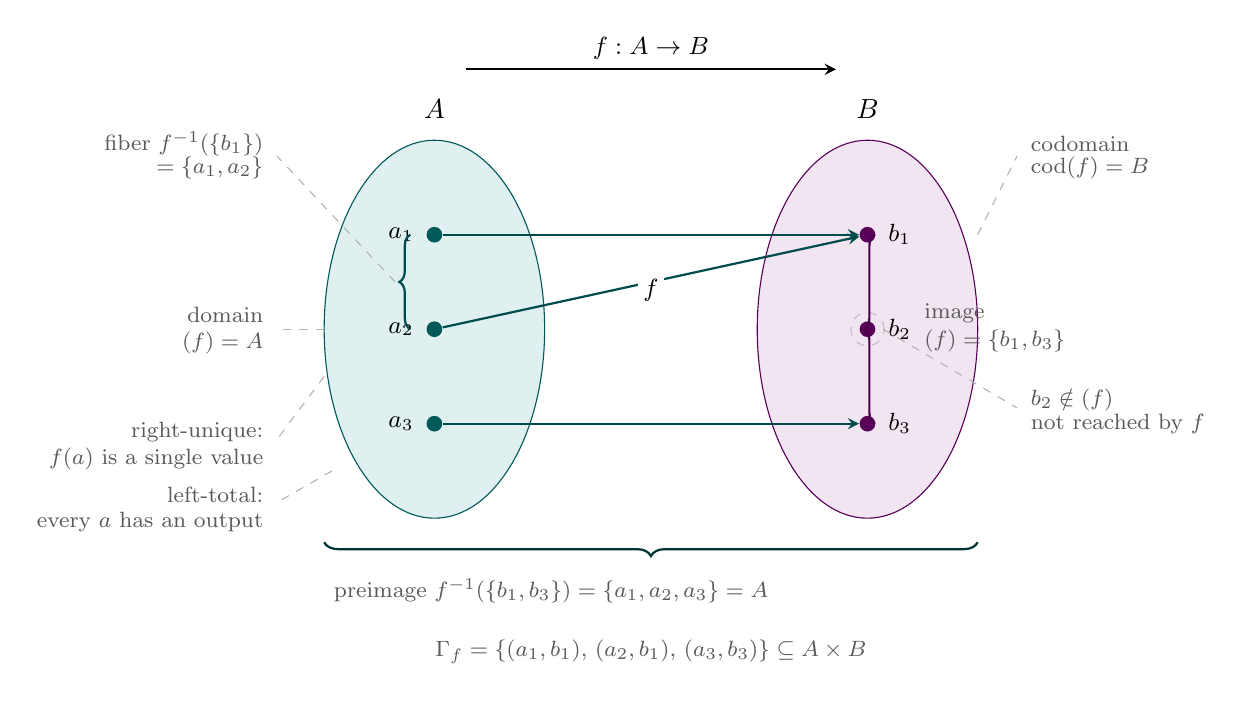
\begin{tikzpicture}[
    >=stealth,
    dot/.style     = {circle, fill, inner sep=2pt},
    teal/.style    = {draw=teal!70!black,  fill=teal!12},
    purple/.style  = {draw=violet!70!black, fill=violet!10},
    lbl/.style     = {font=\small},
    ann/.style     = {font=\footnotesize, text=gray!70!black},
    leader/.style  = {gray!60, dashed, thin},
    arr/.style     = {->, thick, teal!60!black},
    brace/.style   = {decorate,
                      decoration={brace, amplitude=4pt, raise=3pt},
                      thick, violet!60!black}
  ]

  % --- blobs ---
  \draw[teal]   (0,0)   ellipse (1.4cm and 2.4cm);
  \draw[purple] (5.5,0) ellipse (1.4cm and 2.4cm);

  % blob labels
  \node[font=\normalsize\bfseries] at (0,    2.8) {$A$};
  \node[font=\normalsize\bfseries] at (5.5,  2.8) {$B$};

  % --- elements of A ---
  \node[dot, teal!70!black] (a1) at (0,  1.2) {};
  \node[dot, teal!70!black] (a2) at (0,  0)   {};
  \node[dot, teal!70!black] (a3) at (0, -1.2) {};

  \node[lbl, left=4pt] at (a1) {$a_1$};
  \node[lbl, left=4pt] at (a2) {$a_2$};
  \node[lbl, left=4pt] at (a3) {$a_3$};

  % --- elements of B ---
  \node[dot, violet!70!black] (b1) at (5.5,  1.2) {};
  \node[dot, violet!70!black] (b2) at (5.5,  0)   {};
  \node[dot, violet!70!black] (b3) at (5.5, -1.2) {};

  \node[lbl, right=4pt] at (b1) {$b_1$};
  \node[lbl, right=4pt] at (b2) {$b_2$};
  \node[lbl, right=4pt] at (b3) {$b_3$};

  % b2 not in image: dashed ring
  \draw[gray!50, dashed, thin] (b2) circle (6pt);

  % --- arrows ---
  \draw[arr] (a1) -- (b1);
  \draw[arr] (a2) -- (b1);   % two inputs to b1 => not injective
  \draw[arr] (a3) -- (b3);

  % f label on central arrow
  \node[fill=white, inner sep=2pt, font=\small\bfseries] at (2.75, 0.5) {$f$};

  % --- top-level f : A -> B arrow ---
  \draw[->, thick] (0.4, 3.3) -- node[above, font=\small\bfseries] {$f : A \to B$} (5.1, 3.3);

  % ===  LEFT SIDE ANNOTATIONS ===

  % domain
  \draw[leader] (-1.4, 0) -- (-2.0, 0);
  \node[ann, anchor=east] at (-2.05, 0.18) {domain};
  \node[ann, anchor=east] at (-2.05,-0.18) {$\dom(f) = A$};

  % left-total
  \draw[leader] (-1.3,-1.8) -- (-2.0,-2.2);
  \node[ann, anchor=east] at (-2.05,-2.1) {left-total:};
  \node[ann, anchor=east] at (-2.05,-2.45) {every $a$ has an output};

  % right-unique -- left margin, below domain, clear of everything
  \draw[leader] (-1.4, -0.6) -- (-2.0, -1.4);
  \node[ann, anchor=east] at (-2.05,-1.3)  {right-unique:};
  \node[ann, anchor=east] at (-2.05,-1.65) {$f(a)$ is a single value};

  % === RIGHT SIDE ANNOTATIONS ===

  % codomain  -- top right, well clear of image
  \draw[leader] (6.9,  1.2) -- (7.4,  2.2);
  \node[ann, anchor=west] at (7.45, 2.35) {codomain};
  \node[ann, anchor=west] at (7.45, 2.05) {$\mathrm{cod}(f) = B$};

  % image -- mid right, below codomain
  \draw[brace] (5.7, -1.2) -- (5.7,  1.2);
  \node[ann, anchor=west] at (6.1,  0.2) {image};
  \node[ann, anchor=west] at (6.1, -0.15) {$\im(f) = \{b_1, b_3\}$};

  % b2 not in image
  \draw[leader] (5.7, 0) -- (7.4, -1.0);
  \node[ann, anchor=west] at (7.45,-0.9)  {$b_2 \notin \im(f)$};
  \node[ann, anchor=west] at (7.45,-1.2)  {not reached by $f$};

  % fiber of b1: curly brace on LEFT blob, spanning a1 and a2
  \draw[decorate,
        decoration={brace, amplitude=4pt, raise=3pt},
        thick, teal!60!black]
    (-0.2, 0) -- (-0.2, 1.2);
  \draw[leader] (-0.5, 0.6) -- (-2.0, 2.2);
  \node[ann, anchor=east] at (-2.05, 2.35) {fiber $f^{-1}(\{b_1\})$};
  \node[ann, anchor=east] at (-2.05, 2.05) {$= \{a_1, a_2\}$};

  % preimage of T = {b1, b3}  -- bracket under both blobs
  \draw[decorate,
        decoration={brace, amplitude=5pt, raise=3pt, mirror},
        thick, teal!40!black]
    (-1.4,-2.6) -- (6.9,-2.6);
  % label anchored left so it clears the right-unique text
  \node[ann, anchor=north west] at (-1.4,-3.05)
    {preimage $f^{-1}(\{b_1,b_3\}) = \{a_1,a_2,a_3\} = A$};

  % graph label
  \node[ann] at (2.75,-4.1)
    {$\Gamma_f = \{(a_1,b_1),\,(a_2,b_1),\,(a_3,b_3)\} \subseteq A \times B$};

\end{tikzpicture}
\caption{Vocabulary of a function $f : A \to B$.
  Arrows show $f(a_1)=f(a_2)=b_1$ and $f(a_3)=b_3$.
  The element $b_2$ is not in the image; its fiber is empty.
  The fiber over $b_1$ has two elements, showing $f$ is not injective.}
\label{fig:function-vocabulary}
\end{figure}